% !TeX root = ../main.tex
% Add the above to each chapter to make compiling the PDF easier in some editors.

\chapter{Gait Assessment}\label{chapter:gait}

This chapter examines the gait assessment question. We train two models one using the 2D joint estimates as input and one using the 3D joint estimates as input. For each gait video that we have we estimate 28 gait statistics. Gait characteristics need to be understood in a 3D context since they require reasoning about

\section{Data Preprocessing}

The 2D pose output of Open-pose is given in the JSON format. We preprocessed the files to select the pose of the person to the right of the frame. 

\section{Network design}

The gait model is a multi layered Bidirectional Recurrent Neural Networks \parencite{schuster1997bidirectional} which uses Long-Short-Term-Memory (LSTM) \parencite{hochreiter1997long} cells with recurrent dropout \parencite{semeniuta2016recurrent}. In the last layer of the network it contains a fully connected layer which combines information from all the time steps to estimate the output. Each video is used to estimate 28 gait statistics which constitute one row in the Z-matrix. For the network visualization please look at \autoref{fig:gait-network}

\begin{figure}[htpb]
    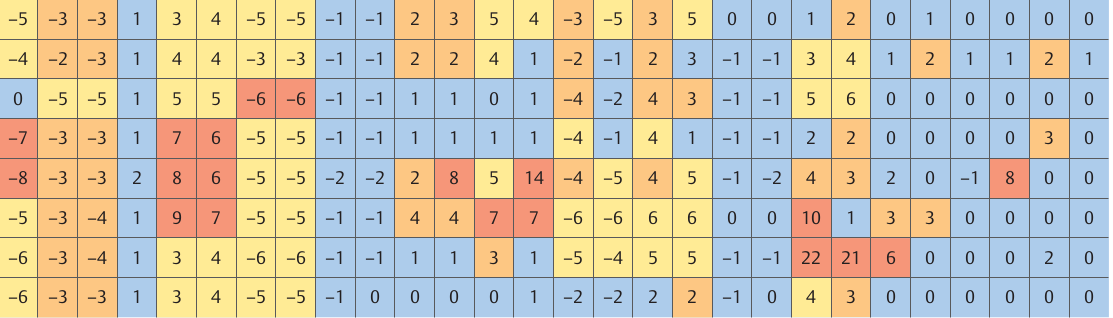
\includegraphics[width=\linewidth]{zmatrix.png}
    \caption{Architecture of the Gait Network}
    \label{fig:gait-network}
\end{figure}

\subsection{Training details}

We train our model for 100 epochs using batch size of 32. We found the sequence length of 256 to be effective. We use the ADAM optimizer with learning rate 0.001

\subsection{Loss Function}

Our model estimates 28 gait statistics $Z \in R^{28}$ given the 2D pose $X \in R^{2\times N}$ or 3D pose 2D pose $\hat{\theta} \in R^{3\times N}$ . We can represent the neural network which takes 3D pose as input as a function $f(\hat{\theta}) = Z ; x \in R^{3\times N}, y \in R^{28} $. As the loss function we use the L-2 norm between the predicted gait statistics and the ground truth gait statistics.

\begin{equation}	
    L(f(\hat{\theta}),Z) = \frac{1}{3N} \cdot \sum_{i=1}^{3N} {\Vert f(\hat{\theta}_i)-Z_i \Vert}_2^2
\end{equation}

When the input is the 2D pose we can define the function as  $f(x) = y ; x \in R^{2\times N}, y \in R^{28} $. Similarly the loss function in this case can be defined as

\begin{equation}	
    L(f(x),Z) = \frac{1}{2N} \cdot \sum_{i=1}^{2N} {\Vert f(x_i)-Z_i \Vert}_2^2
\end{equation}

\section{Evaluation}

For the input 2D and 3D pose sequences are evaluated and compared. The problem is solved as a regression problem by estimating the gait statistics.

\subsection{Results}

For the comparison of the results please look at \autoref{tab:gait-compare}

\begin{table}[htpb]
    \centering
    \begin{tabular}{l l l l}
        \toprule
            A & B & C & D \\
        \midrule
            1 & 2 & 1 & 2 \\
            2 & 3 & 2 & 3 \\
        \bottomrule
    \end{tabular}
    \caption[Comparison Gait]{Compare the gait parameter estimation results between 2D and 3D pose inputs}\label{tab:gait-compare}
\end{table}

\subsection{Discussion of results}

